\chapter{Augmented Foster-Lyapunov Bounds}
In many cases, researchers are interested in the \emph{long-run} behavior of \acp{MPM}.
This behavior is characterized by the stationary distribution of the underlying \ac{CTMC}.
Rigorous analyses of the stationary distribution either hinge on bounds on the moments of this distribution or a Foster-Lyapunov analysis \parencite{kuntz2021stationary}.
Using the former, i.e.\ moment bounds, entails solving a \acl{SDP} involving linear constraints dictated by the moment dynamics.\turnto{sec:moments_bg}
These moment problems are prone to numerical problems because moments increase by several orders of magnitudes with their orders.
Since --~in most cases~-- constraints up to high moment orders are necessary, solving such convex problems is often difficult in practice.
This problem becomes particularly problematic, if some species tend to have high abundances at stationarity.
Reasoning over the drift is often less plagued by numerical issues than the moment bounding approach.
The use of Foster-Lyapunov approaches, is often two-fold: They are used to prove ergodicity and to provide sets with a lower bound $1-\epsilon$ on their stationary probability mass.
Often practical methods focus on proving \emph{global} properties of their associated drift \parencite{gupta2014scalable,spieler2014numerical}.
In many models, simple affine functions \parencite{gupta2017finite} and even the identity \parencite{spieler2014numerical} is sufficient.
While such simple forms provide some of the necessary ease of a global analysis, the task of optimizing them with performance in mind, is much more difficult \parencite{milias2014optimization}.\marginpar{\emph{Performance} in this context means least states to cover most stationary probability mass.}

Ideally one would have the best of both worlds: The ease of working with simple forms for the global guarantees of the Foster-Lyapunov criteria and the freedom of choice to fit efficient functions and get sets that are as small as possible.
The approach presented in this chapter achieves this by \emph{locally} altering a proposal Foster-Lyapunov function.
This proposal function is essentially assumed as an input for this method.
Such a function can be identified by convex analysis, for example \parencite{gupta2014scalable}.
Using a set of probability $>1-\epsilon$ is identified using such a functional.
On this set, the original function is then replaced by any other lower bounded function.
At the set boundary this supplementary function is \emph{phased out} and we switch back to the original function using some smooth step function.
The choice of such a supplementary function offers much room for experimentation since all the necessary global criteria.
For this function we can, for example, use any polynomial or even more variable models such as neural networks.

The procedure to identify an efficient function is thereby reduced to a simple machine learning problem.
The objective exponentially rewards negative drift yielding tight sets.
Its computation needs, in principle, all points in a sufficiently large set.
For optimization however, we switch to an approach of sampling uniformly from the augmentation set.

This method yields sets that are smaller on the order of $10^3$ for a fixed probability bound over a simple linear functional.
We study neural networks and polynomial templates as candidates for local augmentation.

\section{The Drift and its Properties}
The drift \eqref{eq:drift} plays a central role in this chapter.\marginpar{We explain the interpretation and give some basic use of the drift in \autoref{sec:statagg:lyapunov} on page~\pageref{sec:statagg:lyapunov}.}
\begin{equation}
	d(x; g) = Qg(x) = \sum_{j=1}^{n_R} \alpha_j(x) (g(x+v_j) -  g(x))
\end{equation}
An interesting fact about the drift is, that it is invariant to linear transforms to $g$.
That is
\begin{equation}
	Q(g + b)(x)
	=Qg(x)
\end{equation}
for some constant $b\in\mathbb{R}$.
Clearly a positive linear factor $m$ to $g$ factors out, i.e.\ $Q(f\circ g)(x)=mQg(x)$ for $f(x) = mx$, $m>0$.
Consequently, if the drift is scaled by its maximum value, the scaled version is invariant to linear
transforms of $g$:
\begin{equation}
	\frac{Q(f\circ g)(x)}{\max_{x\in\mathcal{S}}Q(f \circ g)(x)}
	=
	\frac{Qg(x)}{\max_{x\in\mathcal{S}}Qg(x)}
\end{equation}
Since the probability bounded sets $C_{\epsilon_{\ell}}$ depend on the scaled drift.
Therefore invariance under linear transformation implies that we cannot change --~especially improve~-- the tightness of the sets by such a transform.

\begin{example}
What makes the perfect Foster-Lyapunov function?
\marginpar{The beauty standard may vary for other applications.}
The confidence interval for level $1-\alpha$ of a Poisson with rate $\mu$ is
\[
\frac{1}{2}P^{-1}(\alpha/2; 2k)\le\mu\leq\frac{1}{2}P^{-1}(1-\alpha/2;{2k+2})\,.
\]
where $P^{-1}(\,\cdot\,; l)$ is the inverse \ac{CDF} of a $\chi^2_{l}$ distribution.
Thus, its the inverse of the regularized gamma function
\[
	\frac{1}{\Gamma(k/2)}\int_0^{x/2} t^{k/2 - 1} e^{-t}\,dt
\]
w.r.t.\ $x$.
	This gives us the ``ideal'' intervals $[l_{\epsilon},h_{\epsilon}]$, $(l_{\epsilon},h_{\epsilon})\in\mathbb{N}^2$ such that
	$\pi_{\infty}([l_{\epsilon},h_{\epsilon}])=1-\epsilon$. These sets are given as the dark area in \autoref{fig:lya_sets}.
Therefore, the perfect Lyapunov function would coincide with those sets. That is,
a function $g$ such that
\[
%	\left\{x\in\mathcal{S}\mid \frac{\epsilon}{c}Qg(x)> \epsilon - 1\right\}
	C_{\epsilon}
	=
	\left[l_{\epsilon}, h_{\epsilon}\right], \quad \forall\epsilon> 0\,.
\]
\end{example}

\section{Augmentation via Local Substitution}
We use a proved Foster-Lyapunov function as a starting point.
For many relevant reaction networks, simple choices such as L1 or L2 norms are sufficient choices \parencite{spieler2014numerical}.
The resulting sets, however, are typically very large.
Tasks such as computing approximate stationary distributions on truncations set up according to these sets can be very costly.
This cost is exacerbated when a system has to be solved for a lot of different reentry matrices, which is necessary when state-wise bounds on the probability conditioned on a truncation are desired~\parencite{dayar2011bounding}.

We propose to augment the proposal function by a function, that is limited to local influence guided by the initial set.
This supplementary function is phased out asymptotically using a simple sigmoid threshold function
\begin{equation}\label{eq:threshold}
  \gamma_{k,z}(x) = \frac{1}{1+k\exp(-x - y)}\,.
\end{equation}
Thus, in a one-dimensional model the augmented Lyapunov $g'$ function becomes
\begin{equation}\label{eq:thres_lyapunov}
    g'(x) = \gamma_{k,z}(x) g(x) + (1 - \gamma_{k,z}(x)) g^*(x)\,.
\end{equation}
The threshold function $\gamma$ guarantees that $g^*$ vanishes asymptotically.
The drifts $d'$ and $d^*$ are defined accordingly.

\begin{example}
Consider the example of Model~\ref{model:bd}.
Using a simple L2 norm as an initially, i.e.\ $g(x) = x^2$, we obtain a fairly large set.
In Figure~\ref{fig:bd:truncation}, we contrast this result to the solution given by the choice of $g^*(x)=(x - 250)^2$, which gives a much tighter subset with the same guarantees.
In this case, the guarantee is that the sets contain at least 0.9 stationary probability mass.
We further demonstrate how the incorporation $g^*$ into $g$ significantly tightens the set proposed initially.
\begin{figure}[htb]
    \centering
    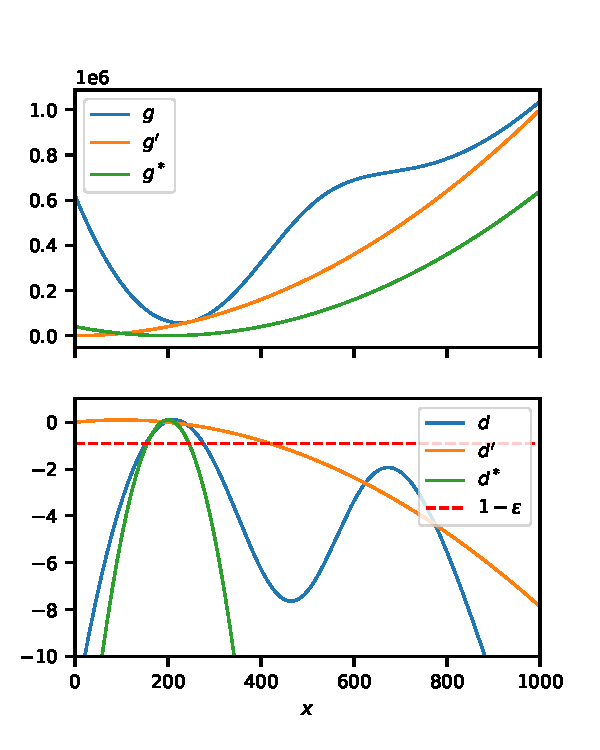
\includegraphics[width=.6\textwidth]{gfx/lyapunov_bd.pdf}
    \caption[Manually augmented Foster-Lyapunov function]{\label{fig:bd:truncation}Different example Lyapunov functions for Model~\ref{model:bd}. The drifts $d$, $d^*$, and $d'$ are scaled and the appropriate threshold for $\epsilon=0.1$ is given.}
\end{figure}
\end{example}


The benefit of the threshold-based construction \eqref{eq:thres_lyapunov} is that we only require $g^*$ to be non-negative.
All other properties are inherited from the proposal function.
This freedom enables the use of flexible machine learning models to search an efficient $g^*$.

\begin{figure}[htb]
\centering
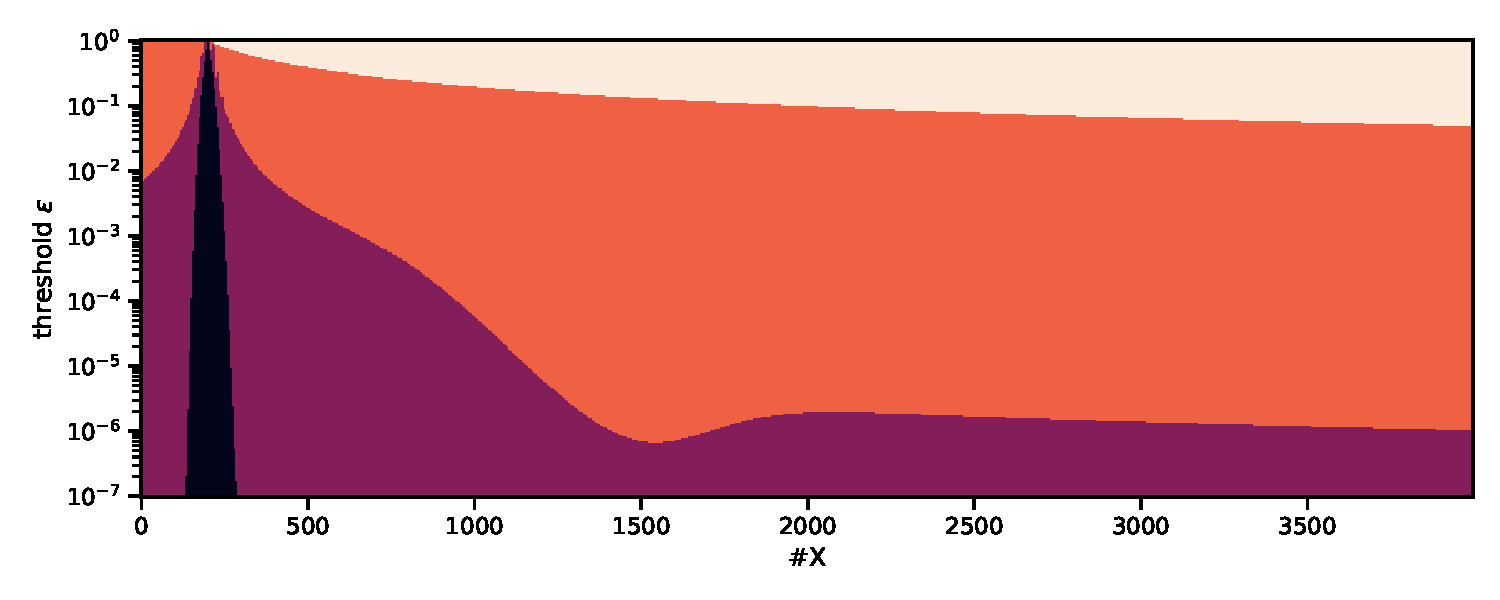
\includegraphics[width=\textwidth]{gfx/lya_sets.pdf}
	\caption[Augmented v.\ proposal Lyapunov sets]{\label{fig:lya_sets}Lyapunov sets for the birth-death process for different probability thresholds $\epsilon$ for the augmented function (red) and the proposal (orange). The ``perfect'' sets are computed using the confidence interval (dark).}
\end{figure}
\begin{figure}[htb]
	\centering
	\subfloat[Linear proposal]
	{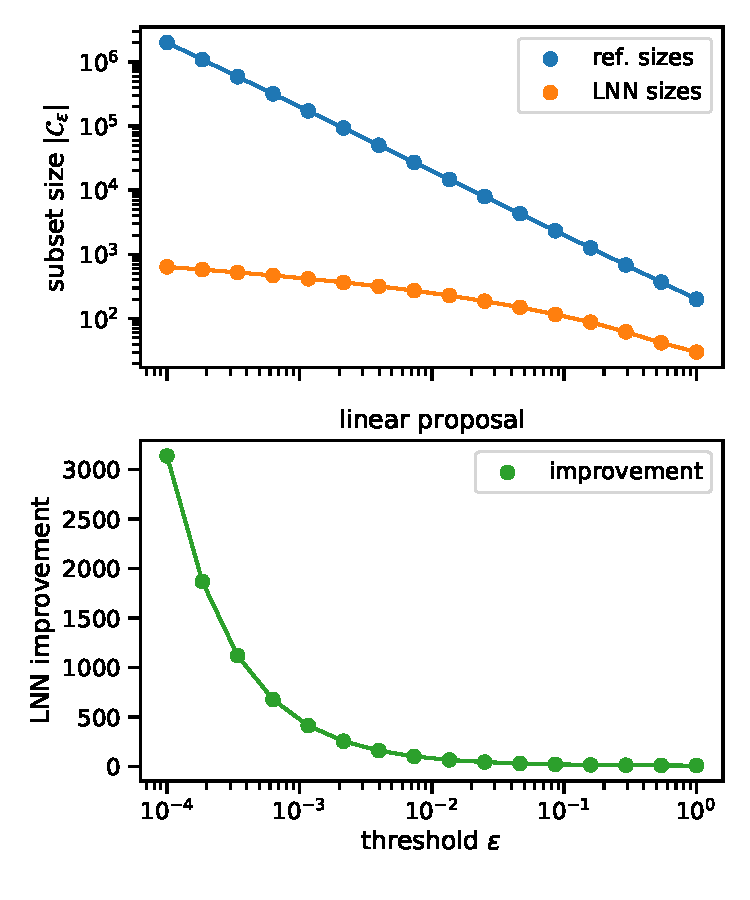
\includegraphics[width=0.48\textwidth]{gfx/lnn_improvement_linear.pdf}}
	\subfloat[Quadratic proposal]
	{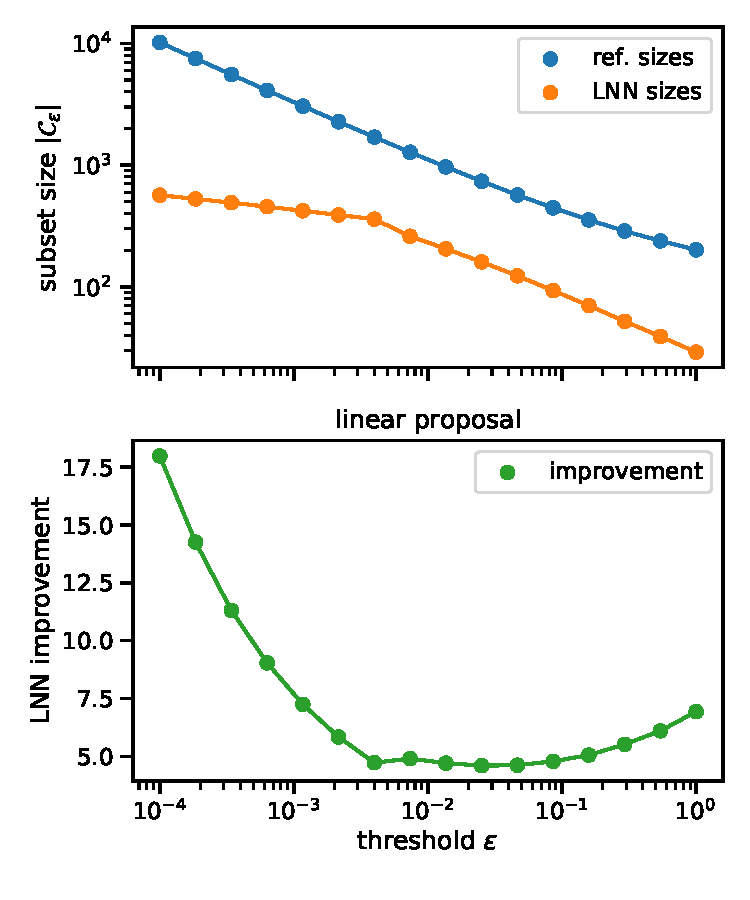
\includegraphics[width=0.48\textwidth]{gfx/lnn_improvement_quadratic.pdf}}
	\caption{\label{fig:improvement}}
\end{figure}

\section{Polynomial Augmentation}

\section{Neural Augmentation}
The characteristics of the augmentation function $g^*$ are typically not known beforehand.
The formulation of augmented Foster-Lyapunov functions only places basic constraints on the function used:
The function needs to be non-negative and an upper bound of the drift has to be known.
Neural networks lend themselves naturally as an extremely flexible functional family.

The central piece of fitting $g^*$ is an objective function.
Since the actual sets, bounded in probability, are defined in terms of their drift, this objective needs to be a function of this drift.
A desirable augmented drift has tight level sets with more emphasis placed on its peak regions.
A natural way to express this prioritization is the objective
\[\sum_{x\in\mathcal{S}}\int_{-\infty}^{d^*(x)}\exp(y)\,dy = \sum_{x\in\mathcal{S}} \exp(d'(x)) \]
based on the scaled augmented drift.

\begin{model}[Competitive Spread]
	Two uncoupled parallel birth-death processes (cf.~\autoref{model:par_bd})\turnto{model:par_bd} supplemented with two Gray-Scott type reactions.
%	https://groups.csail.mit.edu/mac/projects/amorphous/GrayScott/
$$\varnothing\xrightarrow{\rho} A \qquad A\xrightarrow{\delta} \varnothing \qquad
\varnothing\xrightarrow{\rho} B \qquad B\xrightarrow{\delta} \varnothing$$
$$
	2A+B\xrightarrow{\nu_1}3A\qquad
	2A+A\xrightarrow{\nu_2}3B
$$
	As a parameterization we choose $\rho = 5$, $\delta=0.1$, $\nu_1=\e{6}{-5}$, and $\nu_2=\e{6.2}{-5}$.
\end{model}
